This section aims to provide some understanding to Next Generation Sequencing (NGS), the hierarchical structure of data, the quality measurements which are collected when sequencing a sample and how the machines work. All information presented here have been attained from \href{https://support.illumina.com/}{Illuminas website (\today)} (machine manufacturer), through discussion with technicians at the SNP\&SEQ platform or otherwise as cited. 

Next Generation Sequencing (NGS) was introduced in 2005, \citet{NGS}. As described in \citet{NATUREseq}, NGS is a collection of approaches or work flows containing library preparation and sequencing. Here, we will only consider one sequencing procedure, sequencing by synthesis (SBS), which Illumina's machines use. The general work flow with SBS follows the steps seen in Table \ref{NGSWorkFlow} with accompanying Figure \ref{Workflowww}. These two provide a simplification of what is presented in \citet{NGS}. 
\begin{table}[!ht]
\caption{The general workflow using sequencing by synthesis.\label{NGSWorkFlow}}
\begin{enumerate}
\item Library preparation - the DNA sample is randomly fragmented and then prepared for placement on a plate (flowcell).
\item Cluster generation or amplification - the prepared library is loaded onto a plate (flowcell) which has some special features. 
These features together with what is called solid-phase amplification make it possible to clone each fragment placed on the flowcell such that each fragment results in a cluster.
\item Sequencing - the flowcell is placed inside the machine where the sequencing can begin using the SBS technology. 
\item Alignment \& data analysis - the sequenced data and quality variables are extracted. 
\end{enumerate}
\end{table}

The two first steps, library preparation and cluster generation, is performed manually or by a machine. The third step where the sequencing is performed, constitutes of a process where of one of four fluorescent-labelled nucleotides binding to their complementary base pair, contained in the DNA fragment on the flowcell. This process results in a florescent light which can be captured by a camera in the machine. There is a trade-off between cluster generation and sequencing performance. To much cluster generation results in over-clustering and the machine can not distinguish which florescent light appear. On the other hand, a to small amount of cluster generation results in under-clustering and the machine can not detect the florescent light properly.
 
 %There are four steps in sequencing. In short, one first prepares the sample by suitable procedures and thereafter, it is placed on a flowcell. While the prepared sample is on the flowcell we amplify it, creating large clusters of what we want to sequence. This is done in order to increase the ability of the machine to see what is actually on the flowcell. There is a trade-off between how large amplification should be performed and the actual performance of the machine. At the SNP\&SEQ platform these procedures are performed by a human and/or a machine. It all depends on the sample. \textit{No information on who has done what exists}. The sequencing is done by taking pictures of the flowcell at different stages in process. With the help of the created clusters, the bases in the photographs are more easily distinguishable since with the help of these they light up more .........................

Each flowcell has 8 lanes and each of these lanes can provide two reads. Figure \ref{HirStructure} illustrates this hierarchical structure of a flowcell. The measurements made on a lane will in general be worse for Read 2. The camera in the machine emits a light in each step of the sequencing procedure. This light will damage the sample placed on the flowcell. The second reason is that the sequencing procedure takes time. The second read can be performed up to two or three days after the run was started. The quality of the sample can will deteriorate under the sequencing procedure because of the amount of time it is inside the machine. 

Each read provides a measurement of the same cluster but from opposite directions. Between each read, the fragments which are to be sequenced, turns 180 degrees. We can therefore interpret it as read 1 sequence the DNA fragment from the top to the bottom and read 2 sequence the DNA fragment from the bottom to the top. This procedure is performed by the machine with the help of a set of chemicals. The procedure is not deterministic and alignment errors can occur.

When a client provides their sample, they will also specify a number of settings which is to be taken into account for a run. A client will specify which tags corresponds to a certain sample. A tag corresponds to a sequence of base pairs. A flowcell can provide several observations from each read in a given lane, corresponding to the search for different tags. This is seen in Figure \ref{HirStructure}. The number of observations may differ between flowcells. This is the structure of the lowest level in a flowcell, which we will refer to as a flowcells ''tag level''. A higher level exists and at this level only one observation for each read is provided. We will call this level the ''read level''. The client also specifies the number of cycles and lanes/reads to be used in a run. The cycles represents how many times we are repeating the SBS procedure. A higher cycle number implies a longer run time. For some machines, there is only one cycle setting and for others several.

In Table \ref{VariableTable} we can see the quality variables provided by the machines and the data pipeline at SNP\&SEQ. We list what level they are measured on and a very brief description of them. Tag level measurements can be aggregated, by the mean or sum, to receive their respective variable measurements found on read level. This is true to the first decimal. Notice that the completed run cycles are not equal to the actual setting. Therefore we will make the following assumption. A run which has a specific number of completed run cycles had a cycle setting equal to the largest closest possible run setting. Under this assumption we can deduce what type of cycle setting the run was performed on.
\begin{figure}[!ht]
\centering
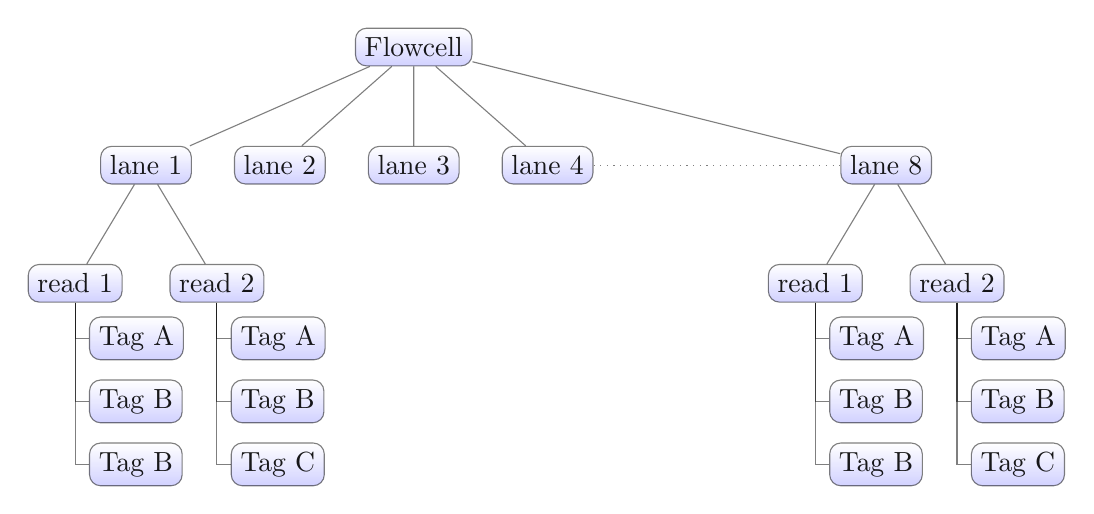
\begin{tikzpicture}[%
	sibling distance=10em,
  	every node/.style = {shape=rectangle, rounded corners,draw,align=center,top color=white, bottom color=blue!20},
    	grandchild/.style={grow=down,xshift=0.5em,anchor=west,
  	  edge from parent path={(\tikzparentnode.south) |- (\tikzchildnode.west)}},
  	grandchildRight/.style={grow=down,xshift=0.5em,anchor=west,
  	  edge from parent path={(\tikzparentnode.south) |-(\tikzchildnode.west)}},
	level 1/.style={sibling distance=17mm},
	level 2/.style={sibling distance=18mm},
	fill opacity=.9,draw opacity=.5
	]
  \node {Flowcell}
    child { node [level 1] (c1) {lane 1} 
    		child [level 2] {node {read 1}
    			child [grandchild, level distance=23mm] { node {Tag B}}	
    			child [grandchild, level distance=15mm] { node {Tag B}}
    			child [grandchild, level distance=7mm] { node {Tag A}}}
    		child [level 2] {node {read 2}
    			child [grandchildRight, level distance=23mm] { node {Tag C}}
    			child [grandchildRight, level distance=15mm] { node {Tag B}}
			child [grandchildRight, level distance=7mm] { node {Tag A}}    		
    		}}
    child [level 1] { node {lane 2} }
	child [level 1] { node {lane 3} }
	child [level 1] { node (c4) {lane 4} }
    child [sibling distance=30mm] { node (c8) {lane 8}
		child [level 2] { node {read 1}
			child [grandchild, level distance=23mm] { node {Tag B}}	
    			child [grandchild, level distance=15mm] { node {Tag B}}
    			child [grandchild, level distance=7mm] { node {Tag A}}}
    		child [level 2] {node {read 2}
    			child [grandchildRight, level distance=23mm] { node {Tag C}}
    			child [grandchildRight, level distance=15mm] { node {Tag B}}
			child [grandchildRight, level distance=7mm] { node {Tag A}}}
    		};
 \draw [dotted] (c4) -- (c8);
		\end{tikzpicture}
 \caption{The hierachical structure of data at the lowest level, tag level, of quality measurement.\label{HirStructure}}
\end{figure}

There are a total of 10 Next Generation Sequencing (NGS) machines of three types (MiSeq, HiSeq2500  and HiSeqX) at the SNP\&SEQ platform. The HiSeqX machines are all of the same model whereas the HiSeq2500 are mixed, upgraded from previous models amongst others. These upgrades do not imply that the machines are equal in terms of their specifications.

Before the NGS machines are used they are cleaned. If a machine is idle for too many days the machine is put through the same maintenance to ensure that it does not deteriorate. It should be noted that the maintenance performed only covers a certain set of parts in the machine such as drain pipes and pumps amongst others. The three different types of machines are generally used for different things. The single MiSeq machine is mainly used for experimental samples. This machine provides less data and the cost of a run is less compared to the others. The MiSeq machine is expected to perform worse since a large portion of variation will be the sample itself. The HiSeq machines are used for common samples and are expected to perform better. They cost more to run but their output is larger. Last, the HiSeqX are the least flexible machines that cost the most to run. These can provide most data amongst the machines and are deemed to be most accurate. 
%When a client is investigating something new or experimental it is often requested to be run on a MiSeq machine. The quality of the sample may be poor because...
\begin{table}[!ht]
\centering
\caption{Table containing quality variables, what level they are measured on and a short description of them. \label{VariableTable}}
\begin{tabular}{lc p{7cm}}
\toprule
Variable & Level & Description \\
\midrule
Mean Q & Tag/Read & The mean quality score of a read \\ 
\midrule
Completed cycles & Tag/Read & Number of completed cycles\\
\midrule
Percent Q30 & Tag/Read & Percentage of base calls which had a Q-value which where over 30 \\ 
\midrule
Error rate & Read & Error rate of read sequence compared to a reference genome  \\ 
\midrule
Percent tag error & Tag & The percent of error of the alignment of this tag \\
\midrule 
Raw cluster & Read & The number of clusters detected in a Read \\ 
\midrule
Past filter Cluster & Tag/Read & The number of clusters detected post filter \\ 
\midrule
Raw Density & Read & The clusters density \\ 
\midrule
Past filter Density & Read & The cluster density, post filter \\
\bottomrule
\end{tabular}
\end{table}

\begin{figure}
\centering
\includegraphics[scale=0.4]{PicSBS.png}
\caption{Figure illustrating the general workflow in sequencing by synthesis. The figure is taken from \citet{NGS}. \label{Workflowww}}
\end{figure}
%The variable \textbf{Mean Q} is the mean of the Phred Q score which is presented in \citet{IlluminaQ}. Without putting to much detail on how the Q score is calculated it is an estimate of how good a cycle is for a specific base. In other words how good the decoding is of a cluster in a picture. As described in Table 1 in the same paper, a Q score of 10 implies a 1 in 10 probability of incorrect base call. A Q score of 30 implies a 1 in 1000 probability of incorrect base call, which is generally deemed as a good and acceptable result. The next variable, completed cycles, is a direct determinant of the machines functionality. Note that these do not represent the actual setting each run was performed on. Since no information was provided on the number of cycles each run was performed on we assume the following; let $R_1$ and $R_2$ represent two cycle settings which suffices $R_1 > R_2$. A run performed on cycle setting $R_1$ can only have at most $R_1$ completed cycles, at least $R_2+1$ completed cycles or zero completed cycles. As an example, a run performed on 126 cycles will have at most 126, at least 102 or 0 completed cycles. A run performed on 101 cycles can at most have 101, at least 52 or 0 completed cycles and so forth. If a run has 0 completed cycles it is assumed to be a malfunction. 

%\textbf{Percent Q30} is the proportion of the sequence of pictures which had a Phred Q score above 30.